\chapter{Implementation}\label{cha:implementation}
\todo[inline]{Implementation på riktig UAV}
\section{System overview}
An overview of the proposed system is shown in Figure \ref{fig:sys_overview}.
\begin{figure}
    \begin{center}
        \begin{tikzpicture}[node distance = 3cm, auto]
            \node[block] (init){Landing area input};
            \node[block, right of=init] (land){Landing sequence calculation};
            \node[block, below of=land] (obst){Obstacle database};
            \node[block, above of=land] (wind){Wind estimation};
            \node[block, right of=land] (mp){Motion planner};
            \node[block, above of=mp] (gps){Positioning system};
            \node[block, right of=mp] (traj){Waypoint controller};

            \path[line] (init) - > node{$\mathcal{A}$} (land); 
            \path[line] (obst) - > node[midway, right]{$\mathcal{X}_{obst}$} (land);
            \path[line] (obst) - > node[midway, right]{$\mathcal{X}_{obst}$} (mp);
            \path[line] (wind) - > node[midway, right]{$\vec{w}$} (land);
            \path[line] (wind) - > node[midway, right]{$\vec{w}$} (mp);
            \path[line] (land) - > node[midway]{$x_f$} (mp);
            \path[line] (gps) - > node[midway, right]{$x_i$} (mp);
            \path[line] (mp) - > node[midway]{$\mathcal{M}$} (traj);
        \end{tikzpicture}
    \end{center}
    \caption{System overview}
    \label{fig:sys_overview}
\end{figure}
The UAV is assumed to be equipped with a wind estimation system which can observe the current wind vector $\vec{w}$, and a positioning system which delivers the current position of the UAV. 
There is also an obstacle database which contains the zones $\mathcal{X}_{obst}$ where the UAV is not allowed to fly. The user inputs a desired landing area $\mathcal{A}$ which is 
used to calculate an landing sequence as described in Chapter \ref{cha:landing}. The resulting approach point is sent as the final state to the motion planner, which calculates a plan from the current 
position received from the positioning system. This plan is then transformed to a waypoint mission $\mathcal{M}$ which is sent for execution to the waypoint controller.
\section{Simulation environment}
The implementation is based on the Ardupilot Software-In-The-Loop (SITL) environment \cite{ardupilot_sitl}. This simulation environment is based on the 
JSBSim simulator \cite{jsbsim}, and is capable of simulating both constant and time-varying wind. The default simulation model is based on the 
Rascal 110 fixed-wing UAV.
\section{Obstacle avoidance}
To ensure low execution times it is crucial to use an efficient method of checking for collisions between states and $\mathcal{X}_{obst}$. 
In this implementation, the S2Geometry library developed by Google was used \cite{s2geo}. This is a C++ library which contains 
efficient methods to index geometrical objects of any shape, and checking for collisions between different geometries such as points, lines and polygons. 
\section{Wind estimation}
\todo[inline]{Skriv mer utförligt om vind-estimering. Eventuellt estimera medelvind och vind-varians online?}
In this thesis the EKF-based wind estimation system described in Section \ref{sec:wind_ekf} was used.
\section{Landing sequence calculation}
In order to calculate the landing sequence the optimization problem \eqref{eq:opt_problem_land} has to be solved. 
This problem was solved using the CasADi toolkit, which is a general toolkit for solving nonlinear optimization problems numerically \cite{casadi}.
\section{Motion planner} 
\subsection{Input set generation}
The input set $\mathcal{U}_s$ is generated using the approach described in Section \ref{sec:motion_prims_wind}. 
It was generated for wind directions $\psi_{w,d}=\{0\degree,20\degree,40\degree,\hdots340\degree\}$ and desired final course 
$\psi_d=\{10\degree,20\degree,\hdots160\degree\}$, resulting in a total of 284 inputs for a specific wind speed $W$. Symmetries of the system mean that inputs
for $\psi_d=\{-10\degree,-20\degree,\hdots-160\degree\}$ are simply found by mirroring the $y_E$ coordinate of $u$.
The optimization problem was solved using NOMAD \cite{nomad}, a C++ implementation of the MADS algorithm. The initial guess for $u$ was defined as 
\begin{equation}
    u_0=(d\cos\psi_d,d\sin\psi_d)
\end{equation}
for the current value of $\psi_d$ and $d=100$ meters. 
Simulations of the closed-loop system for the generated inputs $u$ calculated for some different wind directions and $W=5$ m/s are shown in Figure \ref{fig:motion_prims}.
\begin{figure}
    \begin{center}
        \subfloat[$\psi_w=0\degree$]{
            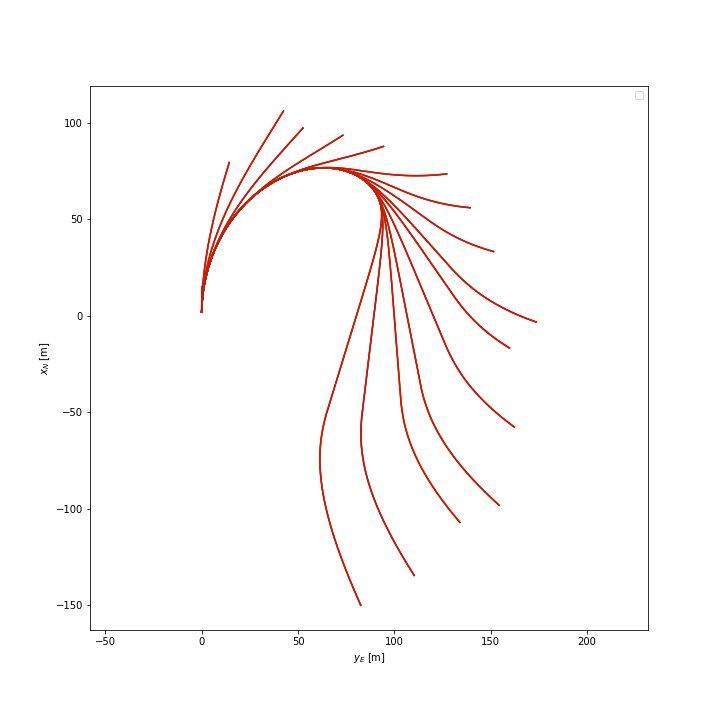
\includegraphics[width=.48\linewidth]{mp_0}
        }
        \subfloat[$\psi_w=80\degree$]{
            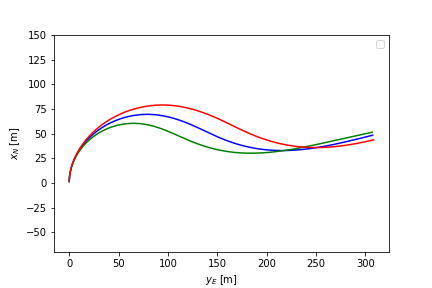
\includegraphics[width=.48\linewidth]{mp_80}
        }
    \end{center}
    \caption{Inputs for different wind directions, $W=5$ m/s}
    \label{fig:motion_prims}
\end{figure}

\subsection{State-space discretization}
To apply graph-search methods the state-space has to be discretized. In this work the values of $x_N$ and $y_E$ were discretized into cells of size $d=10$ meters, and the 
yaw angle $\psi$ was discretized in steps of $20\degree$. The Hybrid $A^*$ method was used when sampling the state space, allowing continuous values of the state vector $x$ but assigning those to the closest 
discretized state.

\subsection{State expansions}
The step $\text{EXPAND}$ in Algorithm \ref{alg:astar} has to take both the wind direction $\psi_w$ and the heading $\psi$ of $x$ into account. 
Since the inputs in $\mathcal{U}_s$ are generated using initial heading $\psi_i=0$, it is first necessary to calculate the closest relative wind direction
\begin{equation}
    \psi_{w,rel}=\argmin_{\psi_{w,d}\in\{\psi_{w,d}\}}|(\psi-\psi_w)-\psi_{w,d}|
\end{equation}
which is used to select the inputs used for expansion. When mirroring inputs the wind direction also has to be mirrored so that 
$\psi_w'=360\degree-\psi_w$. The selected inputs also have to be rotated so that the initial reference $u=(p_{N,g},p_{E,g})$ is transformed to 
\begin{equation}
    u'=(\cos\psi p_{N,g} + \sin\psi p_{E,g}, -\sin\psi p_{N,g} + \cos\psi p_{E,g})
\end{equation}
Finally the expanded states and corresponding costs are found by simulating the closed-loop system \eqref{eq:closed_loop} using each selected $u'$ as input. 
In simulation, the actual wind direction $\psi_w$ is used.
\subsubsection{Handling perpendicular winds}
When expanding states, some inputs become problematic to use when the difference between 
$\psi$ and $\psi_w$ is close to $90 \degree$. In this situation, expanding using an input which corresponds to a heading change 
 of $\Delta\psi\approx180\degree$ might result in the trajectory controller choosing to fly downwind instead of upwind, leading to a large cross track error. This situation is 
 illustrated in Figure \ref{fig:hdg_diff_wind}.

\begin{figure}
    \begin{center}
        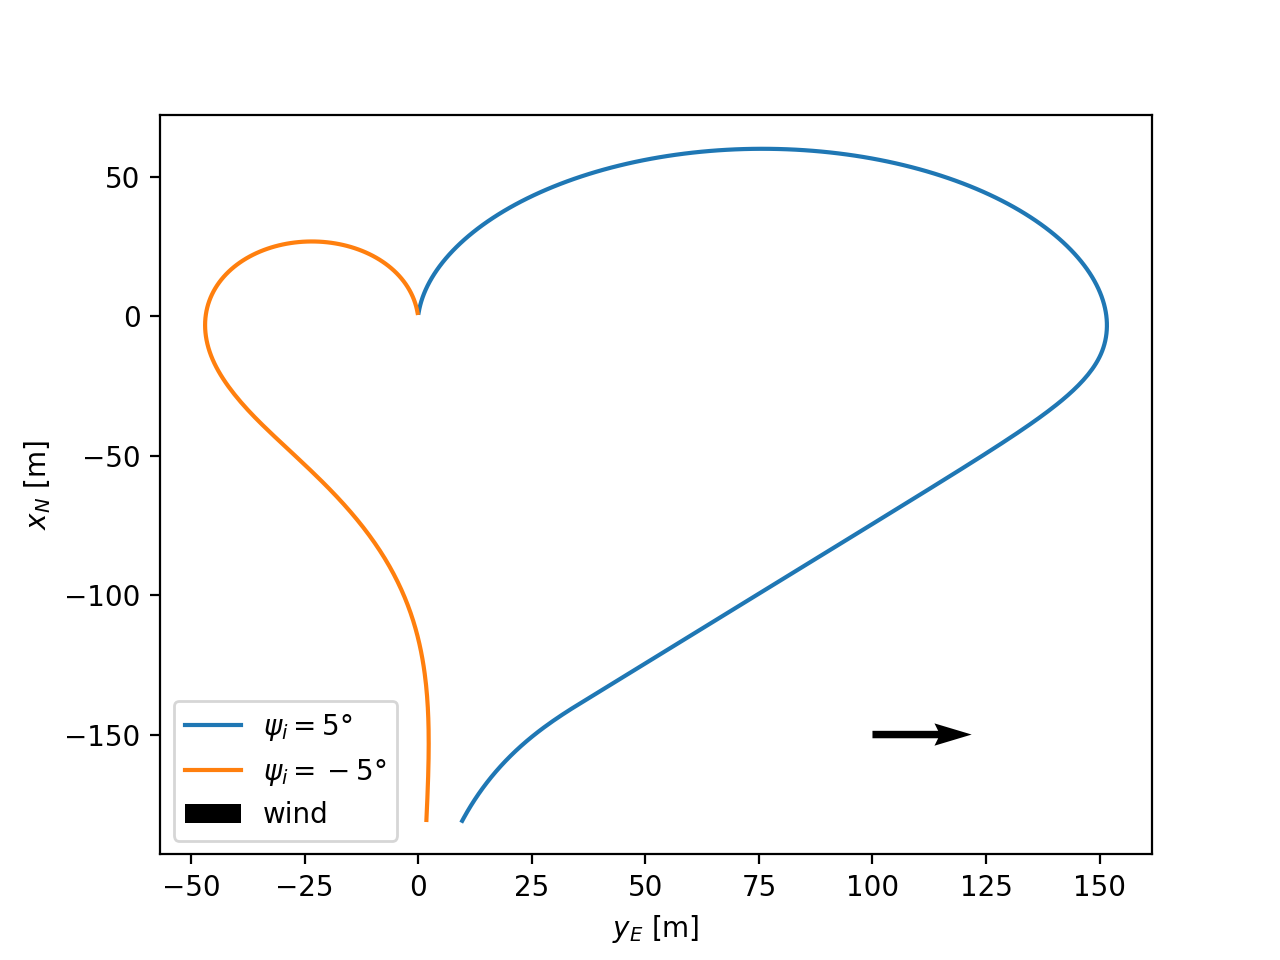
\includegraphics[width=.7\linewidth]{fig/prim_diff_hdg}        
    \end{center}
    \caption{Large cross track error for $\Delta\psi\approx180\degree$ when the wind is perpendicular to UAV motion}
    \label{fig:hdg_diff_wind}
\end{figure}

This issue was handled by defining a set $\psi_{safe}$ defined as 
\begin{equation}
    \psi_{safe}=\{\psi: |\sin\psi|<\frac{1}{\sqrt{2}}\}
\end{equation}
If $|\psi-\psi_w|\notin\psi_{safe}$ during expansion only inputs corresponding to $\Delta\psi\leq160\degree$ are used.

\subsection{Heuristic Lookup Table}
The HLUT was generated using the method in Algorithm \ref{alg:hlut}. The HLUT was generated using the wind-direction $\psi_w=0$, which means that 
entries have to be generated for initial values of $\psi$ from $0\degree$ to $180\degree$ to cover all possibilities. To lookup a query $h(x, x')$ it is then 
necessary to rotate both $x$ and $x'$ by the angle $\psi_w$ in order for the query to align with the HLUT. 

To lower the amount of generated entries the discretization grid was increased to $d=20$ meters when constructing the HLUT. The set of 
values for which to generate entries was selected as 
\begin{equation}
    \mathcal{X}=\{(x_N,y_E): |x_N|\leq D \cup |y_E| \leq D\}
\end{equation}
for $D=400$ m. To ensure that HLUT are entries are available for at least states within a smaller set with $D=200$ m, an additional 
$A^*$ search was performed for each missing such state after the initial generation. For $W=5$ m/s the resulting HLUT consists of 235359 entries. 
A plot of the HLUT values for initial and final heading $\psi_i=\psi_f=0\degree$ can be seen in Figure \ref{fig:hlut}. The dark values at the bottom correspond to where there are no HLUT entries available. 

\begin{figure}
    \begin{center}
        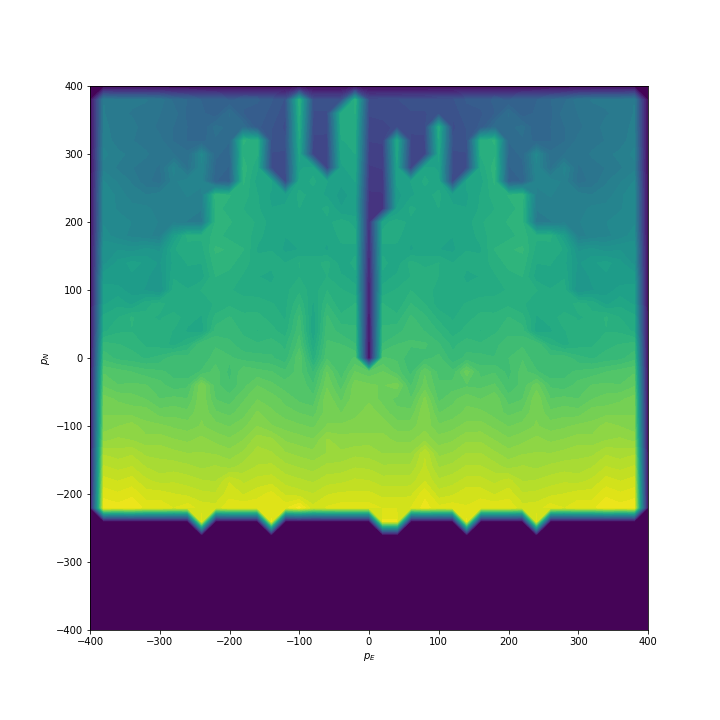
\includegraphics[width=.6\linewidth]{hlut}
    \end{center}
    \caption{HLUT for $W=5$ m/s and $\psi_f=0\degree$}
    \label{fig:hlut}
\end{figure}

\section{Waypoint controller}
To send the calculated motion plan and landing sequence to the waypoint controller, these have to be converted to the 
MAVLink protocol which is supported by the ArduPlane autopilot \cite{mavlink}. This interface was implemented using the MAVROS 
plugin in ROS \cite{mavros}. ROS is a modular framework for robotics applications, with API:s available in both Python and C++ \cite{ros}.
